\chapter{Standard Template Library}

The Standard Template Library (STL) is a collection of C++ template classes that provide general-purpose data structures and algorithms, including \texttt{std::vector}, \texttt{std::list}, \texttt{std::queue}, and \texttt{std::stack}. The STL consists of four main components:

\begin{itemize}
    \item \textbf{Algorithms}: A collection of functions designed to operate on ranges of elements.
    \item \textbf{Containers}: Objects that store collections of other objects.
    \item \textbf{Function Objects}: Components that allow the creation of callable objects.
    \item \textbf{Iterators}: Objects that enable traversal of a container.
\end{itemize}

\section{Containers}

Containers are objects that store data. The STL provides several container classes, each supporting different operations. STL containers are categorized as follows:

\begin{itemize}
    \item \textbf{Sequence Containers}: These containers maintain ordered collections of elements. The main sequence containers are \texttt{std::vector}, \texttt{std::list}, and \texttt{std::deque}.
    \item \textbf{Associative Containers}: These containers store elements in sorted order and support fast searching. The main associative containers are \texttt{std::set}, \texttt{std::multiset}, \texttt{std::map}, and \texttt{std::multimap}.
    \item \textbf{Container Adaptors}: These provide restricted access to elements by adapting existing containers. The primary container adaptors are 	exttt{std::stack}, 	exttt{std::queue}, and 	exttt{std::priority\_queue}.
    \item \textbf{Special Containers}: These containers provide specialized functionality. Examples include \texttt{std::byte}, \texttt{std::pair}, \texttt{std::tuple}, \texttt{std::variant}, \texttt{std::optional} and \texttt{std::any}.
\end{itemize}

\subsection{Sequence Containers}

Sequence containers maintain ordered collections of elements, with element positions independent of their values. In \texttt{std::vector} and \texttt{std::array}, elements are stored contiguously in memory and can be accessed using an index \texttt{[]}.

Examples of sequence containers include \texttt{std::vector<T>}, \texttt{std::array<T,N>}, \texttt{std::deque<T>}, and \texttt{std::list<T>}.

\begin{exampleblock}
    \begin{codeblock}[language=C++]
#include <iostream>
#include <vector>

int main() {
    std::vector<int> v = {1, 2, 3, 4, 5};
    for (int num : v) {
        std::cout << num << " ";
    }
    return 0;
}
    \end{codeblock}
\end{exampleblock}

\subsection{Associative Containers}

Associative containers store elements in sorted order and support fast searching. The main associative containers are \texttt{std::set}, \texttt{std::multiset}, \texttt{std::map}, and \texttt{std::multimap}.

\begin{itemize}
    \item \texttt{std::set} is a container that stores unique elements in sorted order. Here, \textbf{key} and \textbf{value} are the same and thus used interchangeably.
    \item \texttt{std::multiset} is a container that stores multiple elements in sorted order.
    \item \texttt{std::map} is a container that stores key-value pairs in sorted order.
    \item \texttt{std::multimap} is a container that stores multiple key-value pairs in sorted order.
\end{itemize}

\begin{exampleblock}
    \begin{codeblock}[language=C++]
#include <iostream>

int main() {
    std::map<std::string, int> m;
    m["one"] = 1;
    m["two"] = 2;
    m["three"] = 3;

    for (const auto& [key, value] : m) {
        std::cout << key << " => " << value << std::endl;
    }
    return 0;
}
    \end{codeblock}
\end{exampleblock}

They can be further divided in \textbf{ordered} and \textbf{unordered} associative containers. The former maintain elements in sorted order, while the latter do not.
For the former, an ordering relation is required for the elements, which can be provided by a comparison function or by a comparison operator. Moreover, keys can be accessed read-only, but not modified.
For the latter, a hashing function is required for the elements, which can be provided by a hash function or by a hash operator. Keys can be accessed and modified.

\subsection{Container Adaptors}

Container adaptors provide restricted access to elements by adapting existing containers. The primary container adaptors are \texttt{std::stack}, \texttt{std::queue}, and \texttt{std::priority\_queue}.
\begin{itemize}
    \item \texttt{std::stack} is a container that provides a LIFO (Last In, First Out) data structure.
    \item \texttt{std::queue} is a container that provides a FIFO (First In, First Out) data structure.
    \item \texttt{std::priority\_queue} is a container that provides a priority queue data structure.
\end{itemize}

\begin{exampleblock}
    \begin{codeblock}[language=C++]
#include <iostream>
#include <queue>

int main() {
    std::queue<int> q;
    q.push(1);
    q.push(2);
    q.push(3);

    while (!q.empty()) {
        std::cout << q.front() << " ";
        q.pop();
    }
    return 0;
}

    \end{codeblock}
\end{exampleblock}

\subsection{Special Containers}

Special containers provide specialized functionality. Examples include \texttt{std::byte}, \texttt{std::pair}, \texttt{std::tuple}, \texttt{std::variant}, \texttt{std::optional}, and \texttt{std::any}.
\begin{itemize}
    \item \texttt{std::byte} is a container that stores byte values.
    \item \texttt{std::pair} is a container that stores a pair of elements.
    \item \texttt{std::tuple} is a container that stores a tuple of elements.
    \item \texttt{std::variant} is a container that stores a variant of elements.
    \item \texttt{std::optional} is a container that stores an optional value.
    \item \texttt{std::any} is a container that stores any type of value.
\end{itemize}

\begin{exampleblock}
    \begin{codeblock}[language=C++]
#include <iostream>
#include <tuple>

int main() {
    std::tuple<int, float, std::string> t(1
    , 3.14, "Hello");
    std::cout << std::get<0>(t) << " ";
    std::cout << std::get<1>(t) << " ";

    return 0;
}
    \end{codeblock}
\end{exampleblock}

For further examples see \href{https://en.cppreference.com/w/cpp/container}{here}.


\subsection{Iterators}

Iterators are a generalization of \textbf{pointers} that allow a C++ program to work with different data
structures (for example, containers and ranges (since C++20)) in a uniform manner. The iterator
library provides definitions for iterators, as well as iterator traits, adaptors, and utility functions.

\begin{definitionblock}
    An iterator is any object that allows iterating over a succession of elements, typically stored in a
    standard container. It can be dereferenced with the \plaintt{*} operator, returning an element of the
    range, and incremented (moving to the next element) with the \plaintt{++} operator.
\end{definitionblock}

\begin{figure}[H]
    \centering
    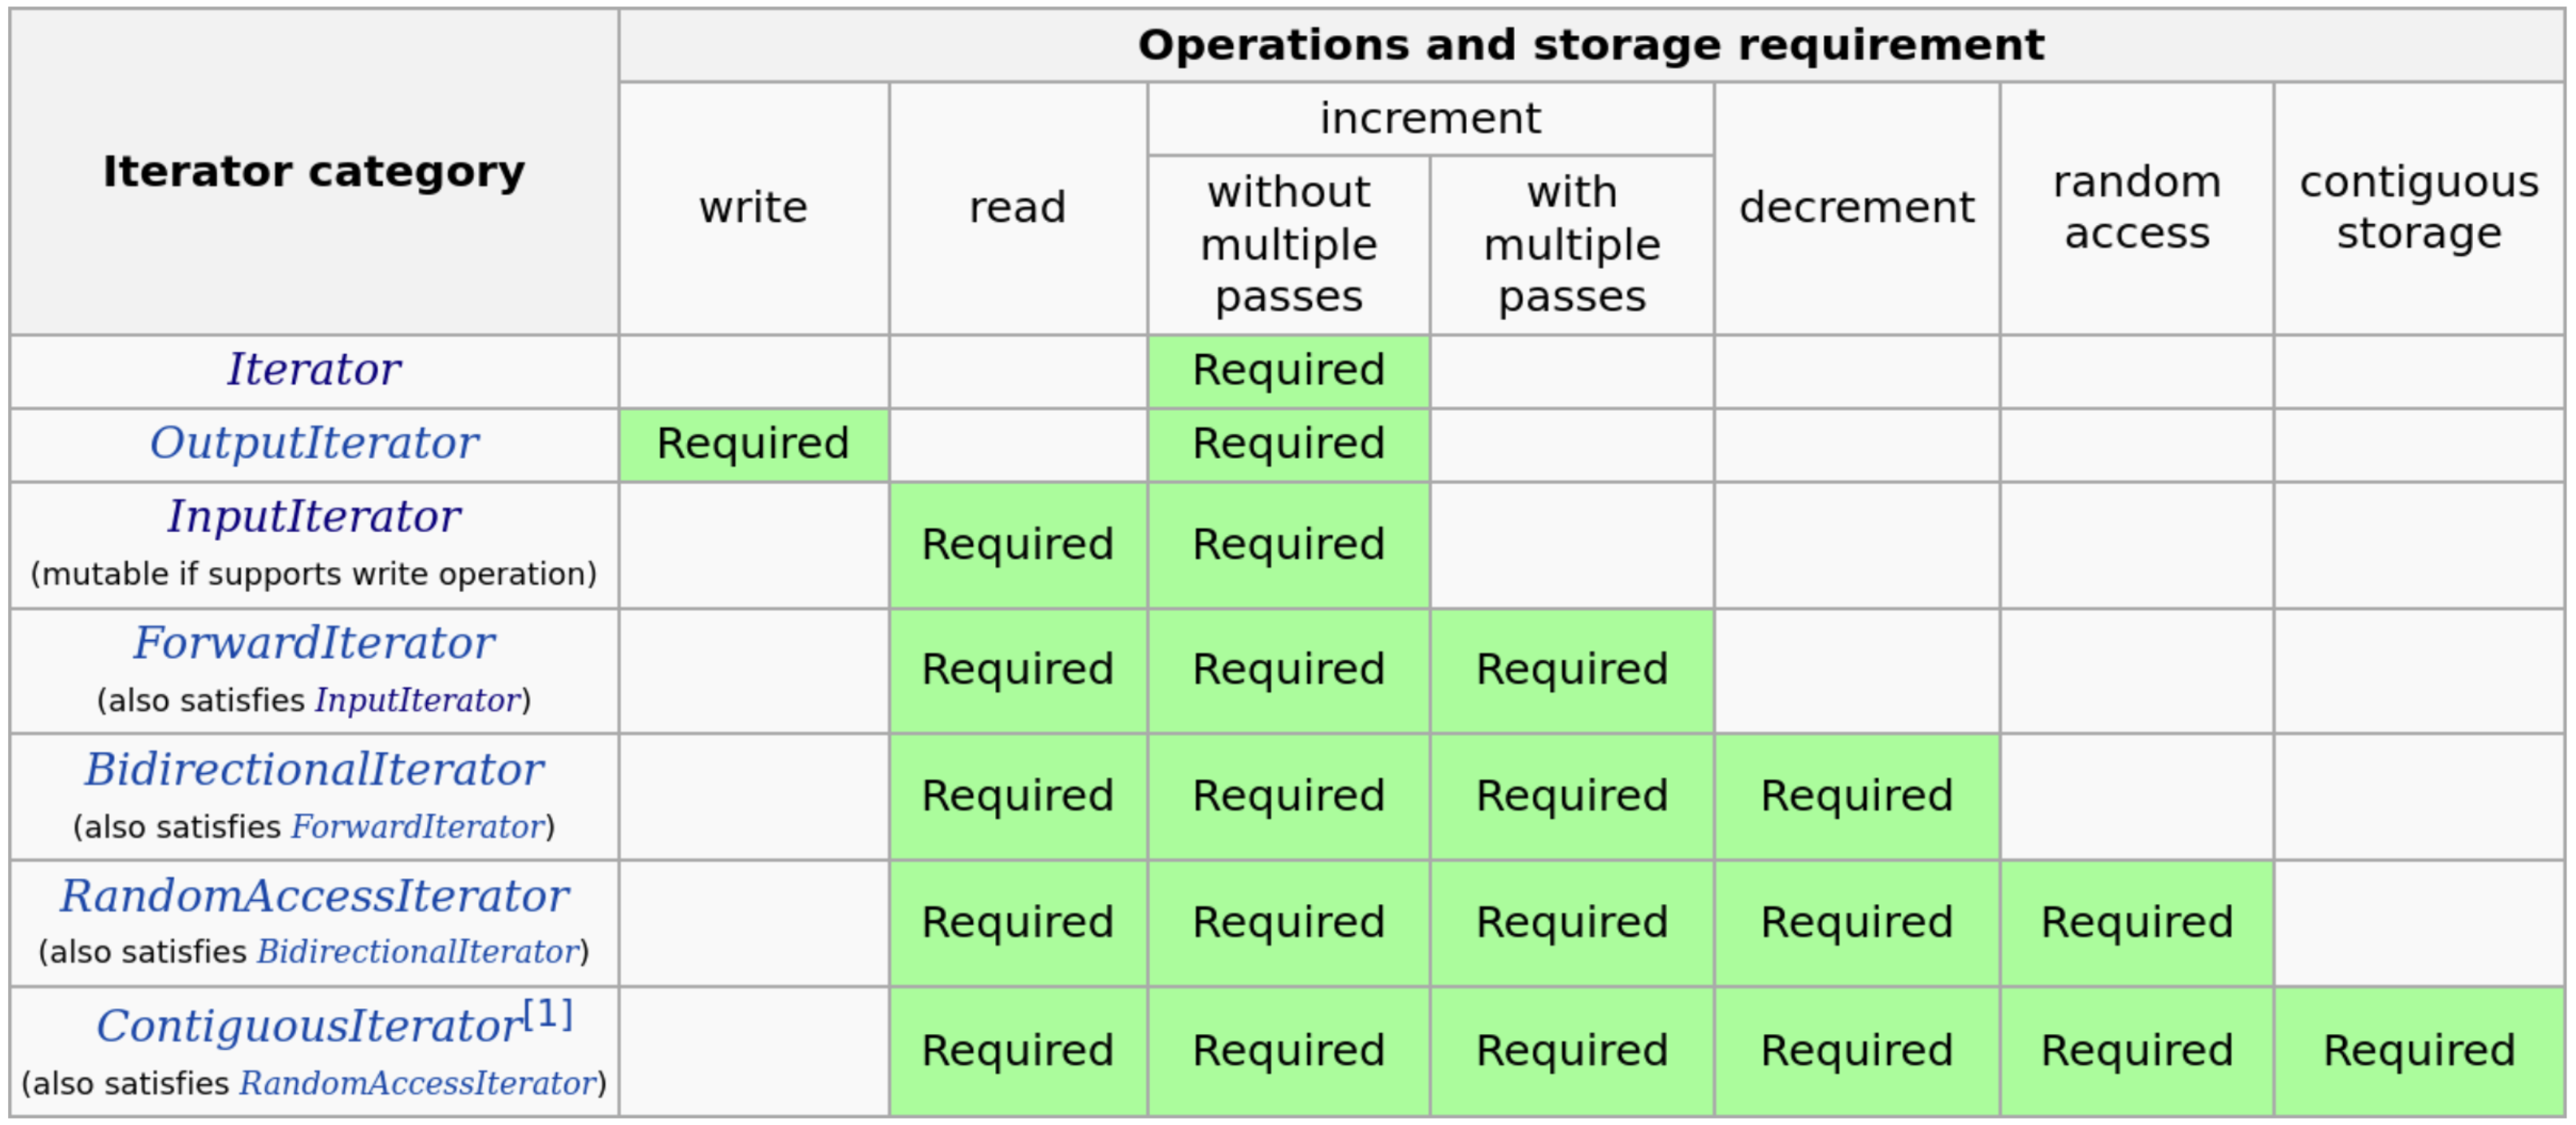
\includegraphics[width=\textwidth]{assets/iterators.png}
    \caption{Iterators}
\end{figure}

\subsection*{Key Concepts of Iterators}
\begin{itemize}
    \item \textbf{Abstraction}: Iterators provide a way to access elements of a container without exposing its internal structure.
    \item \textbf{Uniform Interface}: They offer a consistent interface for traversing different types of containers (e.g., arrays, vectors, lists, etc.).
    \item \textbf{Categories}: Iterators are categorized based on their functionality. The main categories are:
    \begin{itemize}
        \item \textbf{Input Iterators}: Can read elements in a sequence (forward-only, single-pass).
        \item \textbf{Output Iterators}: Can write elements in a sequence (forward-only, single-pass).
        \item \textbf{Forward Iterators}: Can read and write elements in a sequence (forward-only, multi-pass).
        \item \textbf{Bidirectional Iterators}: Can move both forward and backward in a sequence.
        \item \textbf{Random Access Iterators}: Can access any element in constant time (like pointers).
    \end{itemize}
\end{itemize}

\subsection*{Common Iterator Operations}
\begin{itemize}
    \item \texttt{*iter}: Dereference the iterator to access the element it points to.
    \item \texttt{iter->member}: Access a member of the element the iterator points to.
    \item \texttt{++iter} / \texttt{iter++}: Move the iterator to the next element.
    \item \texttt{--iter} / \texttt{iter--}: Move the iterator to the previous element (for bidirectional and random access iterators).
    \item \texttt{iter1 == iter2} / \texttt{iter1 != iter2}: Compare two iterators for equality.
    \item \texttt{iter + n} / \texttt{iter - n}: Move the iterator by \texttt{n} positions (for random access iterators).
\end{itemize}

\subsection*{Iterator Types in C++ Standard Library}
\begin{itemize}
    \item \texttt{begin()} and \texttt{end()}:
    \begin{itemize}
        \item \texttt{begin()} returns an iterator to the first element of the container.
        \item \texttt{end()} returns an iterator to one past the last element (used as a sentinel value).
    \end{itemize}
    \item \texttt{const\_iterator}: A read-only iterator that cannot modify the elements of the container.
    \item \texttt{reverse\_iterator}: Iterates over the container in reverse order.
\end{itemize}
\begin{exampleblock}
\begin{codeblock}[language=C++]
#include <iostream>
#include <vector>

int main() {
    std::vector<int> vec = {1, 2, 3, 4, 5};

    // Using iterators to traverse the vector
    for (auto it = vec.begin(); it != vec.end(); ++it) {
        std::cout << *it << " "; // Dereference the iterator to access the element
    }
    std::cout << std::endl;

    // Using range-based for loop (internally uses iterators)
    for (int val : vec) {
        std::cout << val << " ";
    }
    std::cout << std::endl;

    return 0;
}
\end{codeblock}
\end{exampleblock}

\subsection*{Iterator Categories in Practice}
\begin{itemize}
    \item \textbf{Random Access Iterators}: Supported by \texttt{std::vector}, \texttt{std::array}, and \texttt{std::deque}.
    \item \textbf{Bidirectional Iterators}: Supported by \texttt{std::list} and \texttt{std::set}.
    \item \textbf{Forward Iterators}: Supported by \texttt{std::forward\_list}.
    \item \textbf{Input/Output Iterators}: Used in specific scenarios like reading from or writing to streams.
\end{itemize}

\subsection*{Custom Iterators}
You can also define custom iterators for your own container classes by implementing the required operations (e.g., \texttt{++}, \texttt{*}, \texttt{==}, etc.).

\subsection{size\_type and size\_t}

They are used to represent the size of a container. \texttt{size\_type} is a type defined by the container class, while \texttt{size\_t} is a type defined by the C++ standard library.
They are guaranteed to be unsigned integral types, but their sizes may vary depending on the platform.

\begin{exampleblock}
\begin{codeblock}[language=C++]
#include <iostream>
#include <vector>

int main() {
    std::vector<int> vec = {1, 2, 3, 4, 5};
    std::vector<int>::size_type vec_size = vec.size();
    std::size_t vec_size_t = vec.size();

    std::cout << "size_type: " << vec_size << std::endl;
    std::cout << "size_t: " << vec_size_t << std::endl;

    return 0;
}
\end{codeblock}
\end{exampleblock}

\section{Algorithms}

The STL provides an extensive set of algorithms to operate on containers, or more precisely on
\textbf{ranges}.

\begin{warningblock}
    C++20 has revised the concept of range and provides a new set of algorithms in the
    namespace \plaintt{std::ranges} , with the same name as the old ones, but simpler to use
    and sometimes more powerful.
\end{warningblock}

\subsection*{Why use STL Algorithms?}

With standardized algorithms:
\begin{itemize}
    \item You are more uniform with respect to different container types.
    \item The algorithm of the standard library may do certain optimizations if the contained elements have some characteristics.
    \item You have a parallel version for free$\dots$
\end{itemize}

\subsection{Non-modifying Algorithms}

Non-modifying algorithms do not change the contents of the container (the value in the range). They are used to perform operations like searching, counting, and comparing elements.

\begin{exampleblock}
\begin{codeblock}[language=C++]
#include <iostream>
#include <vector>
#include <algorithm>

int main() {
    std::vector<int> vec = {1, 2, 3, 4, 5};

    // Find the first element greater than 3
    auto it = std::find_if(vec.begin(), vec.end(), [](int x) { return x > 3; });

    if (it != vec.end()) {
        std::cout << "First element greater than 3: " << *it << std::endl;
    }

    // Check if all elements are positive
    bool all_positive = std::all_of(vec.begin(), vec.end(), [](int x) { return x > 0; });

    if (all_positive) {
        std::cout << "All elements are positive" << std::endl;
    }

    return 0;
}
\end{codeblock}
\end{exampleblock}

\subsection{Modifying Algorithms}

Modifying algorithms change the contents of the container. They are used to perform operations like sorting, removing elements, and transforming elements.

\begin{exampleblock}
\begin{codeblock}[language=C++]
#include <iostream>
#include <vector>
#include <algorithm>

int main() {
    std::vector<int> vec = {5, 2, 3, 4, 1};

    // Sort the elements in ascending order
    std::sort(vec.begin(), vec.end());

    // Remove the first element
    vec.erase(vec.begin());

    // Transform each element to its square
    std::transform(vec.begin(), vec.end(), vec.begin(), [](int x) { return x * x; });

    for (int val : vec) {
        std::cout << val << " ";
    }
    std::cout << std::endl;

    return 0;
}
\end{codeblock}
\end{exampleblock}

\subsection{Inserters}

Inserters are used to insert elements into a container. The main inserters are:
\begin{itemize}
    \item \texttt{std::back\_inserter}: Inserts elements at the end of a container.
    \item \texttt{std::front\_inserter}: Inserts elements at the beginning of a container.
    \item \texttt{std::inserter}: Inserts elements at a specified position in a container.
\end{itemize}

\begin{exampleblock}
\begin{codeblock}[language=C++]
#include <iostream>
#include <vector>
#include <algorithm>

int main() {
    std::vector<int> vec1 = {1, 2, 3};
    std::vector<int> vec2 = {4, 5, 6};

    // Insert elements from vec2 to vec1
    std::copy(vec2.begin(), vec2.end(), std::back_inserter(vec1));

    for (int val : vec1) {
        std::cout << val << " ";
    }
    std::cout << std::endl;

    return 0;
}
\end{codeblock}
\end{exampleblock}

\subsection{Sorting Algorithms}

Sorting algorithms are used to arrange elements in a specific order. They operate on a range to order it according to an ordering relation. 

\begin{exampleblock}
\begin{codeblock}[language=C++]
#include <iostream>
#include <vector>
#include <algorithm>

int main() {
    std::vector<int> vec = {5, 2, 3, 4, 1};

    // Sort the elements in ascending order
    std::sort(vec.begin(), vec.end());

    for (int val : vec) {
        std::cout << val << " ";
    }
    std::cout << std::endl;

    return 0;
}
\end{codeblock}
\end{exampleblock}

\subsection{Min and Max}

They are used to find the minimum and maximum elements in a range. The functions \texttt{std::min\_element} and \texttt{std::max\_element} return an iterator to the minimum and maximum elements, respectively.

\begin{exampleblock}
\begin{codeblock}[language=C++]
#include <iostream>
#include <vector>
#include <algorithm>

int main() {
    std::vector<int> vec = {5, 2, 3, 4, 1};

    // Find the minimum and maximum elements
    auto min_it = std::min_element(vec.begin(), vec.end());
    auto max_it = std::max_element(vec.begin(), vec.end());

    std::cout << "Min element: " << *min_it << std::endl;
    std::cout << "Max element: " << *max_it << std::endl;

    return 0;
}
\end{codeblock}
\end{exampleblock}

\subsection{Numeric Algorithms}

Numeric algorithms are used to perform numeric operations on a range of elements. The main numeric algorithms are:

\begin{itemize}
    \item \texttt{std::accumulate}: Computes the sum of elements in a range.
    \item \texttt{std::inner\_product}: Computes the inner product of two ranges.
    \item \texttt{std::partial\_sum}: Computes the partial sum of elements in a range.
    \item \texttt{std::adjacent\_difference}: Computes the differences between adjacent elements in a range.
\end{itemize}

\begin{exampleblock}
\begin{codeblock}[language=C++]
#include <iostream>
#include <vector>
#include <numeric>

int main() {
    std::vector<int> vec = {1, 2, 3, 4, 5};

    // Compute the sum of elements
    int sum = std::accumulate(vec.begin(), vec.end(), 0);

    // Compute the partial sum of elements
    std::vector<int> partial_sum(vec.size());
    std::partial_sum(vec.begin(), vec.end(), partial_sum.begin());

    for (int val : partial_sum) {
        std::cout << val << " ";
    }
    std::cout << std::endl;

    return 0;
}
\end{codeblock}
\end{exampleblock}




\section{STL evolution}

The STL has evolved over time, with new features and improvements introduced in each C++ standard. Here are some key changes in the STL from C++11 to C++20:

\begin{itemize}
    \item \textbf{C++11}: Introduced move semantics, lambda expressions, and range-based for loops.
    \item \textbf{C++14}: Added generic lambdas, variable templates, and binary literals.
    \item \textbf{C++17}: Introduced parallel algorithms, \texttt{std::optional}, \texttt{std::variant}, and \texttt{std::any}.
    \item \textbf{C++20}: Added concepts, ranges, coroutines, and \texttt{std::span}.
\end{itemize}

\subsection*{For loop evolution}

The range-based for loop was introduced in C++11 to simplify iteration over containers. It allows you to iterate over a range of elements without using iterators explicitly.

\begin{exampleblock}
\begin{codeblock}[language=C++]
#include <iostream>
#include <vector>

int main() {
    std::vector<int> vec = {1, 2, 3, 4, 5};

    // Using range-based for loop
    for (int val : vec) {
        std::cout << val << " ";
    }
    std::cout << std::endl;

    return 0;
}
\end{codeblock}
\end{exampleblock}


